\lecture{URLs and Images}{22-11-22}{13:00}{Matt \& Co}{RB LT1}

\section*{URLs}
Uniform Resource Locators (URLs), a subset of Uniform Resource Indicators (URIs), allow us to navigate throughout the internet. They take the following form:
\begin{verbatim}
https://port.ac.uk/
http://www.example.com/forum/questions/?tag=networking&order=newest#top
\end{verbatim}
They can be typed into an address bar, hyperlinked (using the \verb|<a> </a>| tags) or used as the \verb|src| attribute on elements.
\begin{figure}[H]
    \centering
    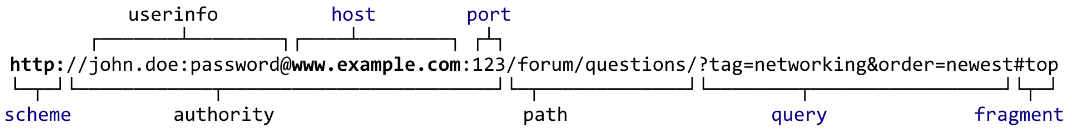
\includegraphics[width=0.9\textwidth]{assets/url-structure.png}
    \caption{URL Structure}
\end{figure}

\subsection*{The \texttt{<a>} tag}
The text between the two tags is what is displayed to the user. The \verb|href| attribute specifies the resource. For example
\begin{html}
<a href="https://www.example.com/">An Example Website</a>
\end{html}
To ensure that the webpages created are accessible to assistive technologies (ie screen readers), do not hyperlink the phrase ``click here'', rather hyperlink a more descriptive phrase for example ``on our website''. 
\subsubsection*{\texttt{target} Attribute}
The \verb|target| attribute can be used to specify \textit{where} to open the link. This can annoy users.
\begin{verbatim}
<a href="https://bbc.co.uk/news" target="_blank">BBC News</a> opens in new tab
\end{verbatim}

\subsection*{URL Types}
Absolute URLs are complete paths to resources, these can be on the same web server or on different web servers.
\begin{verbatim}
/on/the/same/web/server.html
https://on/a/different/web/server.html
\end{verbatim}
Relative URLs refer to resources on the same server. The resource requested is `navigated' to from the current working directory.
\begin{verbatim}
sections/contact.html
../index.html
\end{verbatim}

\subsection*{Fragments}
A fragment can be used to link to a specific part of a page. This can be used to scroll to particular parts of the page. 
\begin{html}
<a href="blurb.html#ch2">Chapter 2</a>
\end{html}
The example above will scroll the browser to the element with the id of \verb|ch2|. 


\section*{Images}
Images are defined using the \verb|<img>| tag. Note that this tag doesn't require a closing tag. A basic, \textit{valid} \verb|<img>| tag requires the \verb|src| and \verb|alt| attributes, to define the source file it will render and alt-text which can be used by screen readers.
\begin{html}
<img
  src="i/elmer/800x400.png"
  alt="a colourful test image."
>
\end{html}

By default, images are displayed at full size. Images can be resized using CSS. For example, to set all images to have width of \verb|30rem| you would use:
\begin{css}
img {
    width: 30rem;
}
\end{css}
The other types of CSS selectors (class, id, etc) can be used for image styling as well.\\

We can use the \verb|float| CSS property to float images to the left or the right of other elements. It is no longer considered best practice to use this method of alignment as the \verb|flex| layout model achieves the same result while being more predictable and controllable.
\subsection*{Captions}
Captions can be added to images as seen below.
\begin{html}
<figure>
  <img
    src="i/teapot.png"
    class="teapot"
    alt="A picture of a tall creamy white porcelain teapot.">

  <figcaption>This is a teapot.</figcaption>
</figure>
\end{html}
\subsection*{Dynamically changing image widths}
In addition to the \verb|src| attribute, we can use the \verb|srcset| attribute to provide a list of alternate images which can be dynamically chosen based on image \& display size. We can add width hints (these come after the file name) which helps the browser select the most appropriate sized image.
\begin{html}
<img
    src="i/logo.png"
    alt="This image has a srcset with width hints."
    srcset="
    i/elmer/400x800.png 400w,
    i/elmer/600x400.png 600w,
    i/elmer/1200x400.png 1200w,
    i/elmer/1600x400.png 1600w,
    i/elmer/3200x400.png 3200w"
>
\end{html}

We can achieve a similar effect using CSS. 

\subsection{An alternative to \texttt{<a>}}
The \verb|<picture>| element allows us to use different images in different situations. It contains multiple \verb|<source>| elements each defining a rule for when it is relevant and then specifies which image to use via its \verb|srcset| attribute.
\begin{html}
<picture>
    <!-- On the biggest screens a large square image  -->
    <source
        media="(min-width: 1600px)"
        srcset="
            i/elmer/800x800.png 1x,
            i/elmer/1600x1600.png 2x,
            i/elmer/3200x3200.png 3x">
    <!-- On smaller screens a sidebar-style image  -->
    <source
        media="(min-width: 800px)"
        srcset="
            i/elmer/200x800.png 1x,
            i/elmer/400x1600.png 2x,
            i/elmer/800x3200.png 3x">
    <!-- Default is a wide masthead shape -->
    <source
        srcset="
            i/elmer/800x200.png 1x,
            i/elmer/1600x400.png 2x,
            i/elmer/3200x800.png 3x">
    <!-- fallback image (required)-->
    <img
        src="i/400x400.png"
        alt="A very dynamic image.">
</picture>
\end{html}

Using the \verb|<picture>| tag also allows us to specify a number of alternative images so that browsers with different capabilities can show their preferred image format
\begin{html}
<picture>
  <source
    type="image/webp"
    srcset="i/uop/logo.webp">
  <source
    type="image/svg+xml"
    srcset="i/uop/logo.svg">
  <source
    type="image/png"
    srcset="i/uop/logo.png">
  <img
    src="i/uop/logo.gif"
    alt="University of Portsmouth Logo">
</picture>
\end{html}


\section*{Videos}
We can include videos in webpages in a similar ways to images. It is best practice to specify multiple formats as for legal reasons not all browsers can support all video formats
\begin{html}
<video
  controls=true
  muted
  style="width: 100%"
  id="v1">
  <source src="i/vid/museum.ogv" type='video/ogv'></source>
  <source src="i/vid/museum.mp4" type='video/mp4'></source>
  <source src="i/vid/museum.mov" type='video/quicktime'></source>
  <p>Sorry, your browser doesn't do video.</p>
</video>
\end{html}